\documentclass[1p]{elsarticle_modified}
%\bibliographystyle{elsarticle-num}

%\usepackage[colorlinks]{hyperref}
%\usepackage{abbrmath_seonhwa} %\Abb, \Ascr, \Acal ,\Abf, \Afrak
\usepackage{amsfonts}
\usepackage{amssymb}
\usepackage{amsmath}
\usepackage{amsthm}
\usepackage{scalefnt}
\usepackage{amsbsy}
\usepackage{kotex}
\usepackage{caption}
\usepackage{subfig}
\usepackage{color}
\usepackage{graphicx}
\usepackage{xcolor} %% white, black, red, green, blue, cyan, magenta, yellow
\usepackage{float}
\usepackage{setspace}
\usepackage{hyperref}

\usepackage{tikz}
\usetikzlibrary{arrows}

\usepackage{multirow}
\usepackage{array} % fixed length table
\usepackage{hhline}

%%%%%%%%%%%%%%%%%%%%%
\makeatletter
\renewcommand*\env@matrix[1][\arraystretch]{%
	\edef\arraystretch{#1}%
	\hskip -\arraycolsep
	\let\@ifnextchar\new@ifnextchar
	\array{*\c@MaxMatrixCols c}}
\makeatother %https://tex.stackexchange.com/questions/14071/how-can-i-increase-the-line-spacing-in-a-matrix
%%%%%%%%%%%%%%%

\usepackage[normalem]{ulem}

\newcommand{\msout}[1]{\ifmmode\text{\sout{\ensuremath{#1}}}\else\sout{#1}\fi}
%SOURCE: \msout is \stkout macro in https://tex.stackexchange.com/questions/20609/strikeout-in-math-mode

\newcommand{\cancel}[1]{
	\ifmmode
	{\color{red}\msout{#1}}
	\else
	{\color{red}\sout{#1}}
	\fi
}

\newcommand{\add}[1]{
	{\color{blue}\uwave{#1}}
}

\newcommand{\replace}[2]{
	\ifmmode
	{\color{red}\msout{#1}}{\color{blue}\uwave{#2}}
	\else
	{\color{red}\sout{#1}}{\color{blue}\uwave{#2}}
	\fi
}

\newcommand{\Sol}{\mathcal{S}} %segment
\newcommand{\D}{D} %diagram
\newcommand{\A}{\mathcal{A}} %arc


%%%%%%%%%%%%%%%%%%%%%%%%%%%%%5 test

\def\sl{\operatorname{\textup{SL}}(2,\Cbb)}
\def\psl{\operatorname{\textup{PSL}}(2,\Cbb)}
\def\quan{\mkern 1mu \triangleright \mkern 1mu}

\theoremstyle{definition}
\newtheorem{thm}{Theorem}[section]
\newtheorem{prop}[thm]{Proposition}
\newtheorem{lem}[thm]{Lemma}
\newtheorem{ques}[thm]{Question}
\newtheorem{cor}[thm]{Corollary}
\newtheorem{defn}[thm]{Definition}
\newtheorem{exam}[thm]{Example}
\newtheorem{rmk}[thm]{Remark}
\newtheorem{alg}[thm]{Algorithm}

\newcommand{\I}{\sqrt{-1}}
\begin{document}

%\begin{frontmatter}
%
%\title{Boundary parabolic representations of knots up to 8 crossings}
%
%%% Group authors per affiliation:
%\author{Yunhi Cho} 
%\address{Department of Mathematics, University of Seoul, Seoul, Korea}
%\ead{yhcho@uos.ac.kr}
%
%
%\author{Seonhwa Kim} %\fnref{s_kim}}
%\address{Center for Geometry and Physics, Institute for Basic Science, Pohang, 37673, Korea}
%\ead{ryeona17@ibs.re.kr}
%
%\author{Hyuk Kim}
%\address{Department of Mathematical Sciences, Seoul National University, Seoul 08826, Korea}
%\ead{hyukkim@snu.ac.kr}
%
%\author{Seokbeom Yoon}
%\address{Department of Mathematical Sciences, Seoul National University, Seoul, 08826,  Korea}
%\ead{sbyoon15@snu.ac.kr}
%
%\begin{abstract}
%We find all boundary parabolic representation of knots up to 8 crossings.
%
%\end{abstract}
%\begin{keyword}
%    \MSC[2010] 57M25 
%\end{keyword}
%
%\end{frontmatter}

%\linenumbers
%\tableofcontents
%
\newcommand\colored[1]{\textcolor{white}{\rule[-0.35ex]{0.8em}{1.4ex}}\kern-0.8em\color{red} #1}%
%\newcommand\colored[1]{\textcolor{white}{ #1}\kern-2.17ex	\textcolor{white}{ #1}\kern-1.81ex	\textcolor{white}{ #1}\kern-2.15ex\color{red}#1	}

{\Large $\underline{10_{105}~(K10a_{72})}$}

\setlength{\tabcolsep}{10pt}
\renewcommand{\arraystretch}{1.6}
\vspace{1cm}\begin{tabular}{m{100pt}>{\centering\arraybackslash}m{274pt}}
\multirow{5}{120pt}{
	\centering
	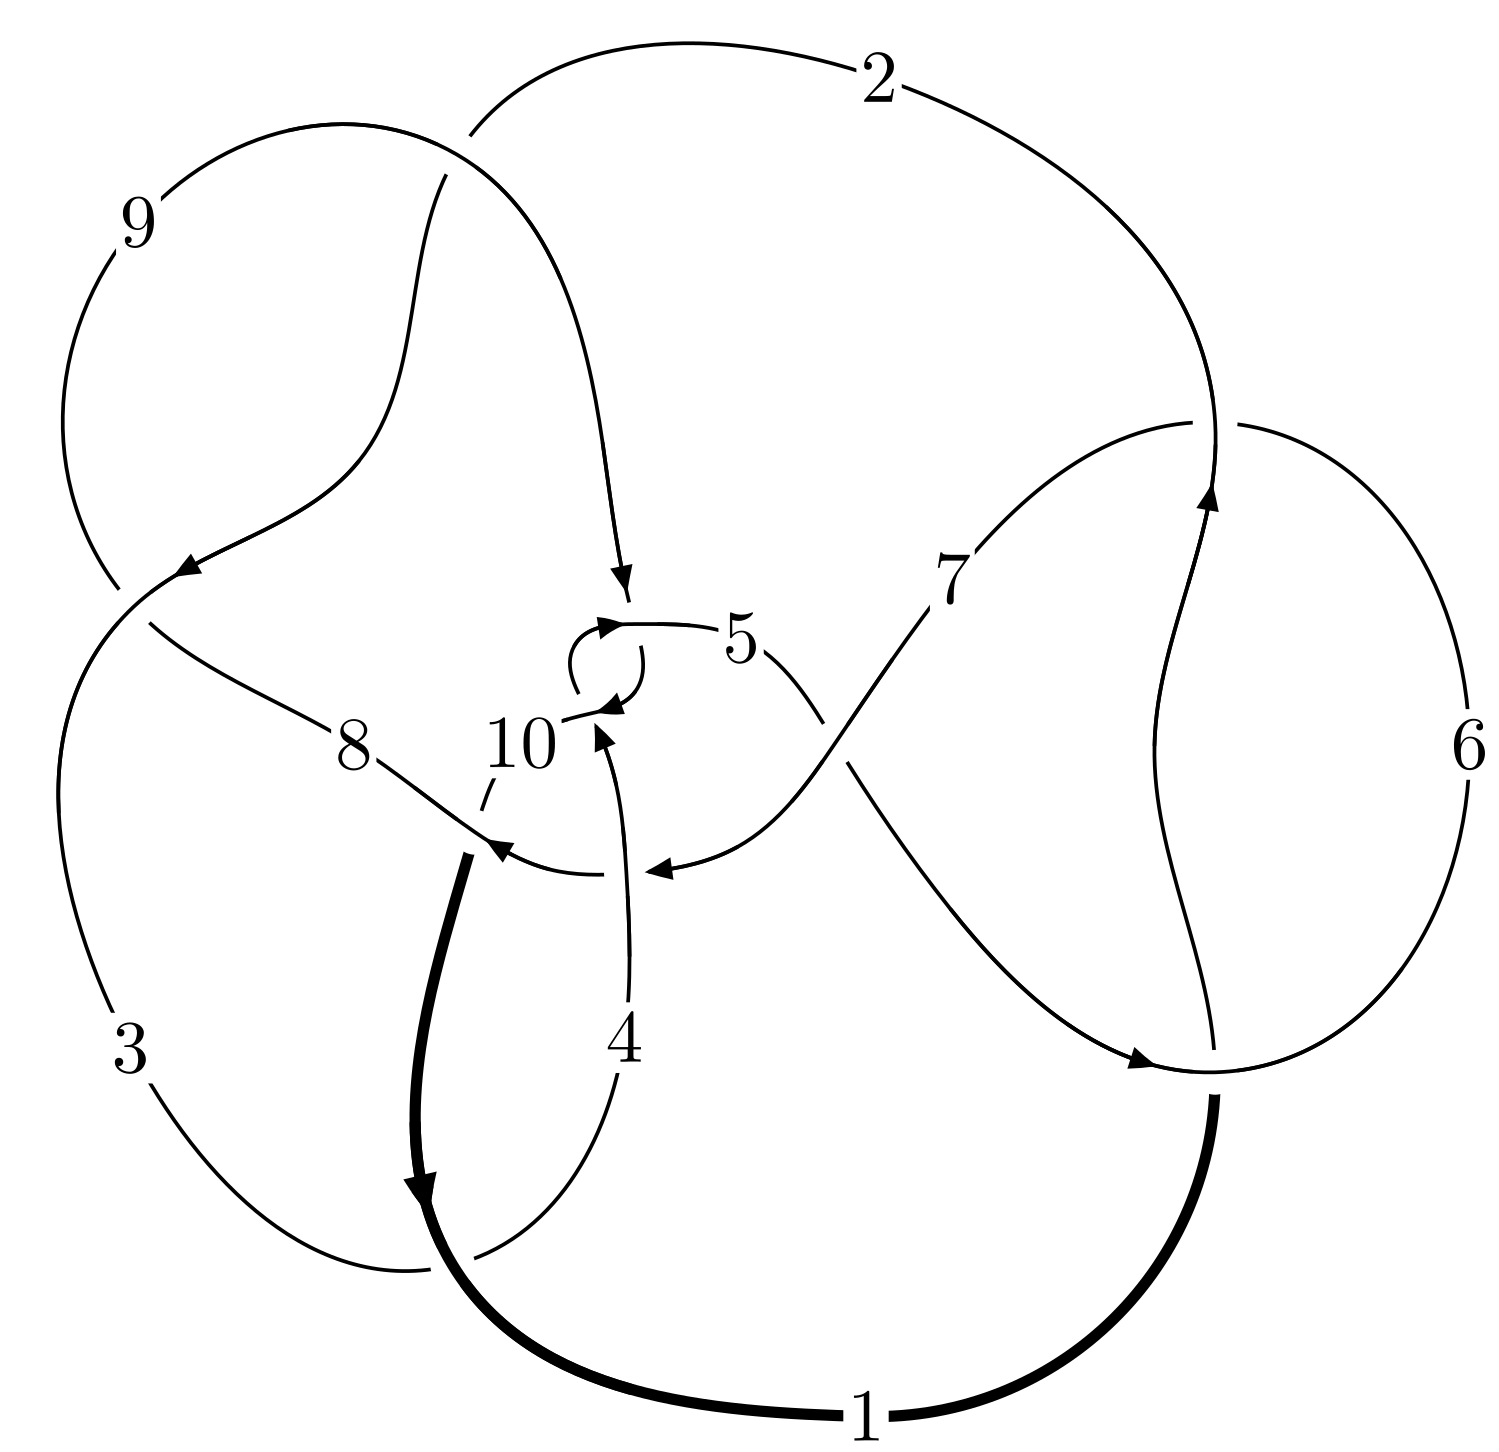
\includegraphics[width=112pt]{../../../GIT/diagram.site/Diagrams/png/189_10_105.png}\\
\ \ \ A knot diagram\footnotemark}&
\allowdisplaybreaks
\textbf{Linearized knot diagam} \\
\cline{2-2}
 &
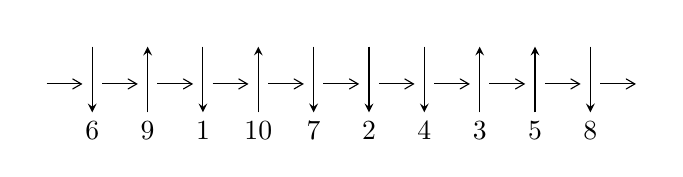
\begin{tikzpicture}[x=20pt, y=17pt]
	% nodes
	\node (C0) at (0, 0) {};
	\node (C1) at (1, 0) {};
	\node (C1U) at (1, +1) {};
	\node (C1D) at (1, -1) {6};

	\node (C2) at (2, 0) {};
	\node (C2U) at (2, +1) {};
	\node (C2D) at (2, -1) {9};

	\node (C3) at (3, 0) {};
	\node (C3U) at (3, +1) {};
	\node (C3D) at (3, -1) {1};

	\node (C4) at (4, 0) {};
	\node (C4U) at (4, +1) {};
	\node (C4D) at (4, -1) {10};

	\node (C5) at (5, 0) {};
	\node (C5U) at (5, +1) {};
	\node (C5D) at (5, -1) {7};

	\node (C6) at (6, 0) {};
	\node (C6U) at (6, +1) {};
	\node (C6D) at (6, -1) {2};

	\node (C7) at (7, 0) {};
	\node (C7U) at (7, +1) {};
	\node (C7D) at (7, -1) {4};

	\node (C8) at (8, 0) {};
	\node (C8U) at (8, +1) {};
	\node (C8D) at (8, -1) {3};

	\node (C9) at (9, 0) {};
	\node (C9U) at (9, +1) {};
	\node (C9D) at (9, -1) {5};

	\node (C10) at (10, 0) {};
	\node (C10U) at (10, +1) {};
	\node (C10D) at (10, -1) {8};
	\node (C11) at (11, 0) {};

	% arrows
	\draw[->,>={angle 60}]
	(C0) edge (C1) (C1) edge (C2) (C2) edge (C3) (C3) edge (C4) (C4) edge (C5) (C5) edge (C6) (C6) edge (C7) (C7) edge (C8) (C8) edge (C9) (C9) edge (C10) (C10) edge (C11) ;	\draw[->,>=stealth]
	(C1U) edge (C1D) (C2D) edge (C2U) (C3U) edge (C3D) (C4D) edge (C4U) (C5U) edge (C5D) (C6U) edge (C6D) (C7U) edge (C7D) (C8D) edge (C8U) (C9D) edge (C9U) (C10U) edge (C10D) ;
	\end{tikzpicture} \\
\hhline{~~} \\& 
\textbf{Solving Sequence} \\ \cline{2-2} 
 &
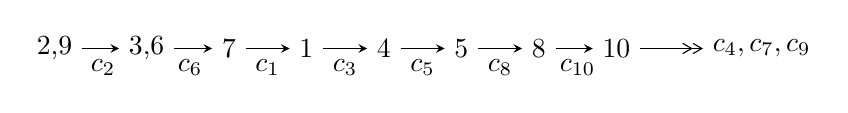
\begin{tikzpicture}[x=28pt, y=7pt]
	% node
	\node (A0) at (-1/8, 0) {2,9};
	\node (A1) at (17/16, 0) {3,6};
	\node (A2) at (17/8, 0) {7};
	\node (A3) at (25/8, 0) {1};
	\node (A4) at (33/8, 0) {4};
	\node (A5) at (41/8, 0) {5};
	\node (A6) at (49/8, 0) {8};
	\node (A7) at (57/8, 0) {10};
	\node (C1) at (1/2, -1) {$c_{2}$};
	\node (C2) at (13/8, -1) {$c_{6}$};
	\node (C3) at (21/8, -1) {$c_{1}$};
	\node (C4) at (29/8, -1) {$c_{3}$};
	\node (C5) at (37/8, -1) {$c_{5}$};
	\node (C6) at (45/8, -1) {$c_{8}$};
	\node (C7) at (53/8, -1) {$c_{10}$};
	\node (A8) at (9, 0) {$c_{4},c_{7},c_{9}$};

	% edge
	\draw[->,>=stealth]	
	(A0) edge (A1) (A1) edge (A2) (A2) edge (A3) (A3) edge (A4) (A4) edge (A5) (A5) edge (A6) (A6) edge (A7) ;
	\draw[->>,>={angle 60}]	
	(A7) edge (A8);
\end{tikzpicture} \\ 

\end{tabular} \\

\footnotetext{
The image of knot diagram is generated by the software ``\textbf{Draw programme}" developed by Andrew Bartholomew(\url{http://www.layer8.co.uk/maths/draw/index.htm\#Running-draw}), where we modified some parts for our purpose(\url{https://github.com/CATsTAILs/LinksPainter}).
}\phantom \\ \newline 
\centering \textbf{Ideals for irreducible components\footnotemark of $X_{\text{par}}$} 
 
\begin{align*}
I^u_{1}&=\langle 
-30 u^{16}-176 u^{15}+\cdots+1103 b+331,\;1294 u^{16}-1159 u^{15}+\cdots+1103 a+2562,\\
\phantom{I^u_{1}}&\phantom{= \langle  }u^{17}+6 u^{15}+u^{14}+16 u^{13}+4 u^{12}+20 u^{11}+7 u^{10}+7 u^9+5 u^8-7 u^7+3 u^6-3 u^5+u^4+3 u^3+2 u+1\rangle \\
I^u_{2}&=\langle 
-4.51865\times10^{39} u^{35}+6.97530\times10^{39} u^{34}+\cdots+1.68010\times10^{40} b-7.80705\times10^{39},\\
\phantom{I^u_{2}}&\phantom{= \langle  }-1.24909\times10^{45} u^{35}+1.82583\times10^{45} u^{34}+\cdots+2.27642\times10^{45} a+4.03057\times10^{46},\\
\phantom{I^u_{2}}&\phantom{= \langle  }u^{36}- u^{35}+\cdots+186 u+43\rangle \\
I^u_{3}&=\langle 
u^6+4 u^4- u^3+4 u^2+b-2 u+2,\;- u^7+u^6-4 u^5+5 u^4-5 u^3+6 u^2+a-3 u+3,\\
\phantom{I^u_{3}}&\phantom{= \langle  }u^8+4 u^6- u^5+5 u^4-2 u^3+4 u^2- u+1\rangle \\
\\
\end{align*}
\raggedright * 3 irreducible components of $\dim_{\mathbb{C}}=0$, with total 61 representations.\\
\footnotetext{All coefficients of polynomials are rational numbers. But the coefficients are sometimes approximated in decimal forms when there is not enough margin.}
\newpage
\renewcommand{\arraystretch}{1}
\centering \section*{I. $I^u_{1}= \langle -30 u^{16}-176 u^{15}+\cdots+1103 b+331,\;1294 u^{16}-1159 u^{15}+\cdots+1103 a+2562,\;u^{17}+6 u^{15}+\cdots+2 u+1 \rangle$}
\flushleft \textbf{(i) Arc colorings}\\
\begin{tabular}{m{7pt} m{180pt} m{7pt} m{180pt} }
\flushright $a_{2}=$&$\begin{pmatrix}1\\0\end{pmatrix}$ \\
\flushright $a_{9}=$&$\begin{pmatrix}0\\u\end{pmatrix}$ \\
\flushright $a_{3}=$&$\begin{pmatrix}1\\- u^2\end{pmatrix}$ \\
\flushright $a_{6}=$&$\begin{pmatrix}-1.17316 u^{16}+1.05077 u^{15}+\cdots+0.526745 u-2.32276\\0.0271985 u^{16}+0.159565 u^{15}+\cdots+1.65549 u-0.300091\end{pmatrix}$ \\
\flushright $a_{7}=$&$\begin{pmatrix}-1.20036 u^{16}+0.891206 u^{15}+\cdots-1.12874 u-2.02267\\0.0271985 u^{16}+0.159565 u^{15}+\cdots+1.65549 u-0.300091\end{pmatrix}$ \\
\flushright $a_{1}=$&$\begin{pmatrix}-0.393472 u^{16}-0.0417044 u^{15}+\cdots+0.317316 u+0.407978\\-1.59383 u^{16}+0.849501 u^{15}+\cdots-0.811423 u-1.61469\end{pmatrix}$ \\
\flushright $a_{4}=$&$\begin{pmatrix}u^2+1\\1.57298 u^{16}-1.10517 u^{15}+\cdots+0.408885 u+1.81142\end{pmatrix}$ \\
\flushright $a_{5}=$&$\begin{pmatrix}-1\\-1.16500 u^{16}+1.49864 u^{15}+\cdots+1.42339 u-0.312783\end{pmatrix}$ \\
\flushright $a_{8}=$&$\begin{pmatrix}- u\\u^3+u\end{pmatrix}$ \\
\flushright $a_{10}=$&$\begin{pmatrix}u\\-1.49864 u^{16}+0.407978 u^{15}+\cdots-1.01723 u-1.16500\end{pmatrix}$\\&\end{tabular}
\flushleft \textbf{(ii) Obstruction class $= -1$}\\~\\
\flushleft \textbf{(iii) Cusp Shapes $= \frac{1215}{1103} u^{16}-\frac{3902}{1103} u^{15}+\cdots+\frac{52}{1103} u-\frac{4030}{1103}$}\\~\\
\newpage\renewcommand{\arraystretch}{1}
\flushleft \textbf{(iv) u-Polynomials at the component}\newline \\
\begin{tabular}{m{50pt}|m{274pt}}
Crossings & \hspace{64pt}u-Polynomials at each crossing \\
\hline $$\begin{aligned}c_{1},c_{6}\end{aligned}$$&$\begin{aligned}
&u^{17}-7 u^{16}+\cdots-36 u+8
\end{aligned}$\\
\hline $$\begin{aligned}c_{2},c_{4},c_{8}\\c_{9}\end{aligned}$$&$\begin{aligned}
&u^{17}+6 u^{15}+\cdots+2 u+1
\end{aligned}$\\
\hline $$\begin{aligned}c_{3},c_{7}\end{aligned}$$&$\begin{aligned}
&u^{17}- u^{16}+\cdots- u+1
\end{aligned}$\\
\hline $$\begin{aligned}c_{5}\end{aligned}$$&$\begin{aligned}
&u^{17}+7 u^{16}+\cdots-48 u+64
\end{aligned}$\\
\hline $$\begin{aligned}c_{10}\end{aligned}$$&$\begin{aligned}
&u^{17}-15 u^{16}+\cdots+608 u-64
\end{aligned}$\\
\hline
\end{tabular}\\~\\
\newpage\renewcommand{\arraystretch}{1}
\flushleft \textbf{(v) Riley Polynomials at the component}\newline \\
\begin{tabular}{m{50pt}|m{274pt}}
Crossings & \hspace{64pt}Riley Polynomials at each crossing \\
\hline $$\begin{aligned}c_{1},c_{6}\end{aligned}$$&$\begin{aligned}
&y^{17}-7 y^{16}+\cdots-48 y-64
\end{aligned}$\\
\hline $$\begin{aligned}c_{2},c_{4},c_{8}\\c_{9}\end{aligned}$$&$\begin{aligned}
&y^{17}+12 y^{16}+\cdots+4 y-1
\end{aligned}$\\
\hline $$\begin{aligned}c_{3},c_{7}\end{aligned}$$&$\begin{aligned}
&y^{17}+3 y^{16}+\cdots-9 y-1
\end{aligned}$\\
\hline $$\begin{aligned}c_{5}\end{aligned}$$&$\begin{aligned}
&y^{17}+5 y^{16}+\cdots+17664 y-4096
\end{aligned}$\\
\hline $$\begin{aligned}c_{10}\end{aligned}$$&$\begin{aligned}
&y^{17}-5 y^{16}+\cdots+17408 y-4096
\end{aligned}$\\
\hline
\end{tabular}\\~\\
\newpage\flushleft \textbf{(vi) Complex Volumes and Cusp Shapes}
$$\begin{array}{c|c|c}  
\text{Solutions to }I^u_{1}& \I (\text{vol} + \sqrt{-1}CS) & \text{Cusp shape}\\
 \hline 
\begin{aligned}
u &= -0.099668 + 0.990377 I \\
a &= \phantom{-}0.755793 + 0.048508 I \\
b &= \phantom{-}0.874913 + 1.017070 I\end{aligned}
 & -0.65585 - 3.58827 I & -5.01554 + 5.19820 I \\ \hline\begin{aligned}
u &= -0.099668 - 0.990377 I \\
a &= \phantom{-}0.755793 - 0.048508 I \\
b &= \phantom{-}0.874913 - 1.017070 I\end{aligned}
 & -0.65585 + 3.58827 I & -5.01554 - 5.19820 I \\ \hline\begin{aligned}
u &= -0.397497 + 1.032420 I \\
a &= \phantom{-}2.04240 - 0.79952 I \\
b &= \phantom{-}1.30568 + 0.56699 I\end{aligned}
 & -3.72641 - 6.77030 I & -4.91686 + 11.50550 I \\ \hline\begin{aligned}
u &= -0.397497 - 1.032420 I \\
a &= \phantom{-}2.04240 + 0.79952 I \\
b &= \phantom{-}1.30568 - 0.56699 I\end{aligned}
 & -3.72641 + 6.77030 I & -4.91686 - 11.50550 I \\ \hline\begin{aligned}
u &= \phantom{-}0.749827 + 0.244567 I \\
a &= \phantom{-}0.108910 + 0.611388 I \\
b &= \phantom{-}0.696825 - 0.650971 I\end{aligned}
 & \phantom{-}2.74501 + 0.69000 I & \phantom{-}3.24547 - 1.78817 I \\ \hline\begin{aligned}
u &= \phantom{-}0.749827 - 0.244567 I \\
a &= \phantom{-}0.108910 - 0.611388 I \\
b &= \phantom{-}0.696825 + 0.650971 I\end{aligned}
 & \phantom{-}2.74501 - 0.69000 I & \phantom{-}3.24547 + 1.78817 I \\ \hline\begin{aligned}
u &= \phantom{-}0.346178 + 0.692637 I \\
a &= -0.666585 + 0.297186 I \\
b &= -0.037067 + 0.756233 I\end{aligned}
 & \phantom{-}0.24233 + 1.64711 I & \phantom{-}1.95019 - 4.12084 I \\ \hline\begin{aligned}
u &= \phantom{-}0.346178 - 0.692637 I \\
a &= -0.666585 - 0.297186 I \\
b &= -0.037067 - 0.756233 I\end{aligned}
 & \phantom{-}0.24233 - 1.64711 I & \phantom{-}1.95019 + 4.12084 I \\ \hline\begin{aligned}
u &= -0.736048 + 0.038467 I \\
a &= \phantom{-}0.755454 + 0.908610 I \\
b &= \phantom{-}0.928563 - 0.638410 I\end{aligned}
 & \phantom{-}2.06897 + 4.31656 I & \phantom{-}2.23828 - 5.03995 I \\ \hline\begin{aligned}
u &= -0.736048 - 0.038467 I \\
a &= \phantom{-}0.755454 - 0.908610 I \\
b &= \phantom{-}0.928563 + 0.638410 I\end{aligned}
 & \phantom{-}2.06897 - 4.31656 I & \phantom{-}2.23828 + 5.03995 I\\
 \hline 
 \end{array}$$\newpage$$\begin{array}{c|c|c}  
\text{Solutions to }I^u_{1}& \I (\text{vol} + \sqrt{-1}CS) & \text{Cusp shape}\\
 \hline 
\begin{aligned}
u &= \phantom{-}0.285508 + 1.357540 I \\
a &= -1.79507 - 0.11101 I \\
b &= -1.375440 - 0.134825 I\end{aligned}
 & -10.04230 + 5.59145 I & -9.61044 - 4.67516 I \\ \hline\begin{aligned}
u &= \phantom{-}0.285508 - 1.357540 I \\
a &= -1.79507 + 0.11101 I \\
b &= -1.375440 + 0.134825 I\end{aligned}
 & -10.04230 - 5.59145 I & -9.61044 + 4.67516 I \\ \hline\begin{aligned}
u &= -0.52629 + 1.31806 I \\
a &= -0.119329 - 0.266115 I \\
b &= \phantom{-}0.352099 - 0.977016 I\end{aligned}
 & -3.89694 - 9.32757 I & -4.13921 + 5.55906 I \\ \hline\begin{aligned}
u &= -0.52629 - 1.31806 I \\
a &= -0.119329 + 0.266115 I \\
b &= \phantom{-}0.352099 + 0.977016 I\end{aligned}
 & -3.89694 + 9.32757 I & -4.13921 - 5.55906 I \\ \hline\begin{aligned}
u &= \phantom{-}0.59743 + 1.42672 I \\
a &= \phantom{-}1.62332 + 0.78900 I \\
b &= \phantom{-}1.192940 - 0.641161 I\end{aligned}
 & -6.4799 + 15.1817 I & -6.31050 - 8.67042 I \\ \hline\begin{aligned}
u &= \phantom{-}0.59743 - 1.42672 I \\
a &= \phantom{-}1.62332 - 0.78900 I \\
b &= \phantom{-}1.192940 + 0.641161 I\end{aligned}
 & -6.4799 - 15.1817 I & -6.31050 + 8.67042 I \\ \hline\begin{aligned}
u &= -0.438874\phantom{ +0.000000I} \\
a &= -1.40978\phantom{ +0.000000I} \\
b &= -0.877026\phantom{ +0.000000I}\end{aligned}
 & -1.63327\phantom{ +0.000000I} & -4.88280\phantom{ +0.000000I}\\
 \hline 
 \end{array}$$\newpage\newpage\renewcommand{\arraystretch}{1}
\centering \section*{II. $I^u_{2}= \langle -4.52\times10^{39} u^{35}+6.98\times10^{39} u^{34}+\cdots+1.68\times10^{40} b-7.81\times10^{39},\;-1.25\times10^{45} u^{35}+1.83\times10^{45} u^{34}+\cdots+2.28\times10^{45} a+4.03\times10^{46},\;u^{36}- u^{35}+\cdots+186 u+43 \rangle$}
\flushleft \textbf{(i) Arc colorings}\\
\begin{tabular}{m{7pt} m{180pt} m{7pt} m{180pt} }
\flushright $a_{2}=$&$\begin{pmatrix}1\\0\end{pmatrix}$ \\
\flushright $a_{9}=$&$\begin{pmatrix}0\\u\end{pmatrix}$ \\
\flushright $a_{3}=$&$\begin{pmatrix}1\\- u^2\end{pmatrix}$ \\
\flushright $a_{6}=$&$\begin{pmatrix}0.548710 u^{35}-0.802063 u^{34}+\cdots-49.1305 u-17.7057\\0.268951 u^{35}-0.415172 u^{34}+\cdots-2.22836 u+0.464678\end{pmatrix}$ \\
\flushright $a_{7}=$&$\begin{pmatrix}0.279759 u^{35}-0.386891 u^{34}+\cdots-46.9021 u-18.1704\\0.268951 u^{35}-0.415172 u^{34}+\cdots-2.22836 u+0.464678\end{pmatrix}$ \\
\flushright $a_{1}=$&$\begin{pmatrix}-0.769505 u^{35}+1.07166 u^{34}+\cdots+31.1795 u+19.4777\\-0.393831 u^{35}+0.112167 u^{34}+\cdots-65.8523 u-14.5725\end{pmatrix}$ \\
\flushright $a_{4}=$&$\begin{pmatrix}-0.637961 u^{35}+0.592755 u^{34}+\cdots-103.303 u-23.1636\\-0.184491 u^{35}+0.149837 u^{34}+\cdots-15.4345 u+1.18486\end{pmatrix}$ \\
\flushright $a_{5}=$&$\begin{pmatrix}-0.359956 u^{35}+0.244025 u^{34}+\cdots-66.5978 u-5.35101\\0.294559 u^{35}-0.557722 u^{34}+\cdots-13.0683 u-4.16067\end{pmatrix}$ \\
\flushright $a_{8}=$&$\begin{pmatrix}- u\\u^3+u\end{pmatrix}$ \\
\flushright $a_{10}=$&$\begin{pmatrix}-0.371740 u^{35}+1.03334 u^{34}+\cdots+105.667 u+33.5297\\-0.291646 u^{35}+0.0216178 u^{34}+\cdots-56.3790 u-13.1684\end{pmatrix}$\\&\end{tabular}
\flushleft \textbf{(ii) Obstruction class $= -1$}\\~\\
\flushleft \textbf{(iii) Cusp Shapes $= -0.228694 u^{35}-0.643530 u^{34}+\cdots-255.696 u-70.7596$}\\~\\
\newpage\renewcommand{\arraystretch}{1}
\flushleft \textbf{(iv) u-Polynomials at the component}\newline \\
\begin{tabular}{m{50pt}|m{274pt}}
Crossings & \hspace{64pt}u-Polynomials at each crossing \\
\hline $$\begin{aligned}c_{1},c_{6}\end{aligned}$$&$\begin{aligned}
&(u^6+u^5- u^4-2 u^3+u+1)^6
\end{aligned}$\\
\hline $$\begin{aligned}c_{2},c_{4},c_{8}\\c_{9}\end{aligned}$$&$\begin{aligned}
&u^{36}- u^{35}+\cdots+186 u+43
\end{aligned}$\\
\hline $$\begin{aligned}c_{3},c_{7}\end{aligned}$$&$\begin{aligned}
&u^{36}-3 u^{35}+\cdots-16 u+1
\end{aligned}$\\
\hline $$\begin{aligned}c_{5}\end{aligned}$$&$\begin{aligned}
&(u^6+3 u^5+5 u^4+4 u^3+2 u^2+u+1)^6
\end{aligned}$\\
\hline $$\begin{aligned}c_{10}\end{aligned}$$&$\begin{aligned}
&(u^3+u^2-1)^{12}
\end{aligned}$\\
\hline
\end{tabular}\\~\\
\newpage\renewcommand{\arraystretch}{1}
\flushleft \textbf{(v) Riley Polynomials at the component}\newline \\
\begin{tabular}{m{50pt}|m{274pt}}
Crossings & \hspace{64pt}Riley Polynomials at each crossing \\
\hline $$\begin{aligned}c_{1},c_{6}\end{aligned}$$&$\begin{aligned}
&(y^6-3 y^5+5 y^4-4 y^3+2 y^2- y+1)^6
\end{aligned}$\\
\hline $$\begin{aligned}c_{2},c_{4},c_{8}\\c_{9}\end{aligned}$$&$\begin{aligned}
&y^{36}+27 y^{35}+\cdots+29904 y+1849
\end{aligned}$\\
\hline $$\begin{aligned}c_{3},c_{7}\end{aligned}$$&$\begin{aligned}
&y^{36}-9 y^{35}+\cdots-36 y+1
\end{aligned}$\\
\hline $$\begin{aligned}c_{5}\end{aligned}$$&$\begin{aligned}
&(y^6+y^5+5 y^4+6 y^2+3 y+1)^6
\end{aligned}$\\
\hline $$\begin{aligned}c_{10}\end{aligned}$$&$\begin{aligned}
&(y^3- y^2+2 y-1)^{12}
\end{aligned}$\\
\hline
\end{tabular}\\~\\
\newpage\flushleft \textbf{(vi) Complex Volumes and Cusp Shapes}
$$\begin{array}{c|c|c}  
\text{Solutions to }I^u_{2}& \I (\text{vol} + \sqrt{-1}CS) & \text{Cusp shape}\\
 \hline 
\begin{aligned}
u &= -1.046060 + 0.100110 I \\
a &= -0.471095 + 0.739312 I \\
b &= -0.428243 - 0.664531 I\end{aligned}
 & -0.02007 + 3.75243 I & -0.77353 - 3.77367 I \\ \hline\begin{aligned}
u &= -1.046060 - 0.100110 I \\
a &= -0.471095 - 0.739312 I \\
b &= -0.428243 + 0.664531 I\end{aligned}
 & -0.02007 - 3.75243 I & -0.77353 + 3.77367 I \\ \hline\begin{aligned}
u &= -0.071145 + 1.052640 I \\
a &= \phantom{-}2.96217 + 0.54442 I \\
b &= \phantom{-}1.002190 - 0.295542 I\end{aligned}
 & -3.80128 - 1.90382 I & -8.20696 + 2.18522 I \\ \hline\begin{aligned}
u &= -0.071145 - 1.052640 I \\
a &= \phantom{-}2.96217 - 0.54442 I \\
b &= \phantom{-}1.002190 + 0.295542 I\end{aligned}
 & -3.80128 + 1.90382 I & -8.20696 - 2.18522 I \\ \hline\begin{aligned}
u &= \phantom{-}0.445481 + 0.807833 I \\
a &= -0.769672 - 0.151793 I \\
b &= -0.428243 + 0.664531 I\end{aligned}
 & -0.02007 + 1.90382 I & -0.77353 - 2.18522 I \\ \hline\begin{aligned}
u &= \phantom{-}0.445481 - 0.807833 I \\
a &= -0.769672 + 0.151793 I \\
b &= -0.428243 - 0.664531 I\end{aligned}
 & -0.02007 - 1.90382 I & -0.77353 + 2.18522 I \\ \hline\begin{aligned}
u &= -0.015491 + 1.101610 I \\
a &= \phantom{-}0.567110 - 0.099771 I \\
b &= -0.428243 - 0.664531 I\end{aligned}
 & -4.15765 + 0.92430 I & -7.30279 - 0.79423 I \\ \hline\begin{aligned}
u &= -0.015491 - 1.101610 I \\
a &= \phantom{-}0.567110 + 0.099771 I \\
b &= -0.428243 + 0.664531 I\end{aligned}
 & -4.15765 - 0.92430 I & -7.30279 + 0.79423 I \\ \hline\begin{aligned}
u &= \phantom{-}0.098878 + 1.131130 I \\
a &= -1.90200 - 0.19672 I \\
b &= -1.073950 + 0.558752 I\end{aligned}
 & -1.91067 + 2.86490 I & -4.49024 - 2.53112 I \\ \hline\begin{aligned}
u &= \phantom{-}0.098878 - 1.131130 I \\
a &= -1.90200 + 0.19672 I \\
b &= -1.073950 - 0.558752 I\end{aligned}
 & -1.91067 - 2.86490 I & -4.49024 + 2.53112 I\\
 \hline 
 \end{array}$$\newpage$$\begin{array}{c|c|c}  
\text{Solutions to }I^u_{2}& \I (\text{vol} + \sqrt{-1}CS) & \text{Cusp shape}\\
 \hline 
\begin{aligned}
u &= -0.196406 + 1.132180 I \\
a &= -1.65820 + 1.54999 I \\
b &= -1.073950 - 0.558752 I\end{aligned}
 & -6.04826 - 5.69302 I & -11.01951 + 5.51057 I \\ \hline\begin{aligned}
u &= -0.196406 - 1.132180 I \\
a &= -1.65820 - 1.54999 I \\
b &= -1.073950 + 0.558752 I\end{aligned}
 & -6.04826 + 5.69302 I & -11.01951 - 5.51057 I \\ \hline\begin{aligned}
u &= \phantom{-}1.031890 + 0.635795 I \\
a &= \phantom{-}0.203148 - 0.430936 I \\
b &= \phantom{-}1.002190 + 0.295542 I\end{aligned}
 & -3.80128 + 1.90382 I & -8.20696 - 2.18522 I \\ \hline\begin{aligned}
u &= \phantom{-}1.031890 - 0.635795 I \\
a &= \phantom{-}0.203148 + 0.430936 I \\
b &= \phantom{-}1.002190 - 0.295542 I\end{aligned}
 & -3.80128 - 1.90382 I & -8.20696 + 2.18522 I \\ \hline\begin{aligned}
u &= \phantom{-}0.444188 + 1.146330 I \\
a &= \phantom{-}0.054279 - 0.572062 I \\
b &= -0.428243 - 0.664531 I\end{aligned}
 & -0.02007 + 3.75243 I & -0.77353 - 3.77367 I \\ \hline\begin{aligned}
u &= \phantom{-}0.444188 - 1.146330 I \\
a &= \phantom{-}0.054279 + 0.572062 I \\
b &= -0.428243 + 0.664531 I\end{aligned}
 & -0.02007 - 3.75243 I & -0.77353 + 3.77367 I \\ \hline\begin{aligned}
u &= -0.560207 + 1.124730 I \\
a &= \phantom{-}1.81411 - 1.13202 I \\
b &= \phantom{-}1.002190 + 0.295542 I\end{aligned}
 & -3.80128 - 3.75243 I & -8.20696 + 3.77367 I \\ \hline\begin{aligned}
u &= -0.560207 - 1.124730 I \\
a &= \phantom{-}1.81411 + 1.13202 I \\
b &= \phantom{-}1.002190 - 0.295542 I\end{aligned}
 & -3.80128 + 3.75243 I & -8.20696 - 3.77367 I \\ \hline\begin{aligned}
u &= -0.598261 + 0.392855 I \\
a &= -0.352723 + 0.385946 I \\
b &= -1.073950 + 0.558752 I\end{aligned}
 & -1.91067 + 2.86490 I & -4.49024 - 2.53112 I \\ \hline\begin{aligned}
u &= -0.598261 - 0.392855 I \\
a &= -0.352723 - 0.385946 I \\
b &= -1.073950 - 0.558752 I\end{aligned}
 & -1.91067 - 2.86490 I & -4.49024 + 2.53112 I\\
 \hline 
 \end{array}$$\newpage$$\begin{array}{c|c|c}  
\text{Solutions to }I^u_{2}& \I (\text{vol} + \sqrt{-1}CS) & \text{Cusp shape}\\
 \hline 
\begin{aligned}
u &= \phantom{-}1.350340 + 0.016723 I \\
a &= -0.597073 - 0.522912 I \\
b &= -1.073950 + 0.558752 I\end{aligned}
 & -1.91067 + 8.52114 I & -4.49024 - 8.49002 I \\ \hline\begin{aligned}
u &= \phantom{-}1.350340 - 0.016723 I \\
a &= -0.597073 + 0.522912 I \\
b &= -1.073950 - 0.558752 I\end{aligned}
 & -1.91067 - 8.52114 I & -4.49024 + 8.49002 I \\ \hline\begin{aligned}
u &= -0.388989 + 1.300350 I \\
a &= -2.16057 + 0.72732 I \\
b &= -1.073950 - 0.558752 I\end{aligned}
 & -1.91067 - 8.52114 I & -4.49024 + 8.49002 I \\ \hline\begin{aligned}
u &= -0.388989 - 1.300350 I \\
a &= -2.16057 - 0.72732 I \\
b &= -1.073950 + 0.558752 I\end{aligned}
 & -1.91067 + 8.52114 I & -4.49024 - 8.49002 I \\ \hline\begin{aligned}
u &= -0.274718 + 0.565739 I \\
a &= -0.544610 + 1.141380 I \\
b &= -0.428243 + 0.664531 I\end{aligned}
 & -0.02007 + 1.90382 I & -0.77353 - 2.18522 I \\ \hline\begin{aligned}
u &= -0.274718 - 0.565739 I \\
a &= -0.544610 - 1.141380 I \\
b &= -0.428243 - 0.664531 I\end{aligned}
 & -0.02007 - 1.90382 I & -0.77353 + 2.18522 I \\ \hline\begin{aligned}
u &= -0.555599 + 1.270020 I \\
a &= \phantom{-}0.035250 - 0.334569 I \\
b &= -0.428243 + 0.664531 I\end{aligned}
 & -4.15765 - 0.92430 I & -7.30279 + 0.79423 I \\ \hline\begin{aligned}
u &= -0.555599 - 1.270020 I \\
a &= \phantom{-}0.035250 + 0.334569 I \\
b &= -0.428243 - 0.664531 I\end{aligned}
 & -4.15765 + 0.92430 I & -7.30279 - 0.79423 I \\ \hline\begin{aligned}
u &= -0.06736 + 1.43539 I \\
a &= \phantom{-}1.81428 - 0.63593 I \\
b &= \phantom{-}1.002190 - 0.295542 I\end{aligned}
 & -7.93886 + 0.92430 I & -14.7362 - 0.7942 I \\ \hline\begin{aligned}
u &= -0.06736 - 1.43539 I \\
a &= \phantom{-}1.81428 + 0.63593 I \\
b &= \phantom{-}1.002190 + 0.295542 I\end{aligned}
 & -7.93886 - 0.92430 I & -14.7362 + 0.7942 I\\
 \hline 
 \end{array}$$\newpage$$\begin{array}{c|c|c}  
\text{Solutions to }I^u_{2}& \I (\text{vol} + \sqrt{-1}CS) & \text{Cusp shape}\\
 \hline 
\begin{aligned}
u &= -0.216323 + 0.422026 I \\
a &= -1.90801 - 1.66447 I \\
b &= \phantom{-}1.002190 - 0.295542 I\end{aligned}
 & -3.80128 + 3.75243 I & -8.20696 - 3.77367 I \\ \hline\begin{aligned}
u &= -0.216323 - 0.422026 I \\
a &= -1.90801 + 1.66447 I \\
b &= \phantom{-}1.002190 + 0.295542 I\end{aligned}
 & -3.80128 - 3.75243 I & -8.20696 + 3.77367 I \\ \hline\begin{aligned}
u &= \phantom{-}0.80839 + 1.45058 I \\
a &= -1.15715 - 0.89131 I \\
b &= -1.073950 + 0.558752 I\end{aligned}
 & -6.04826 + 5.69302 I & \phantom{-0.000000 } 0 \\ \hline\begin{aligned}
u &= \phantom{-}0.80839 - 1.45058 I \\
a &= -1.15715 + 0.89131 I \\
b &= -1.073950 - 0.558752 I\end{aligned}
 & -6.04826 - 5.69302 I & \phantom{-0.000000 } 0 \\ \hline\begin{aligned}
u &= \phantom{-}0.31139 + 1.81407 I \\
a &= \phantom{-}1.280070 - 0.127233 I \\
b &= \phantom{-}1.002190 + 0.295542 I\end{aligned}
 & -7.93886 - 0.92430 I & \phantom{-0.000000 } 0 \\ \hline\begin{aligned}
u &= \phantom{-}0.31139 - 1.81407 I \\
a &= \phantom{-}1.280070 + 0.127233 I \\
b &= \phantom{-}1.002190 - 0.295542 I\end{aligned}
 & -7.93886 + 0.92430 I & \phantom{-0.000000 } 0\\
 \hline 
 \end{array}$$\newpage\newpage\renewcommand{\arraystretch}{1}
\centering \section*{III. $I^u_{3}= \langle u^6+4 u^4- u^3+4 u^2+b-2 u+2,\;- u^7+u^6+\cdots+a+3,\;u^8+4 u^6- u^5+5 u^4-2 u^3+4 u^2- u+1 \rangle$}
\flushleft \textbf{(i) Arc colorings}\\
\begin{tabular}{m{7pt} m{180pt} m{7pt} m{180pt} }
\flushright $a_{2}=$&$\begin{pmatrix}1\\0\end{pmatrix}$ \\
\flushright $a_{9}=$&$\begin{pmatrix}0\\u\end{pmatrix}$ \\
\flushright $a_{3}=$&$\begin{pmatrix}1\\- u^2\end{pmatrix}$ \\
\flushright $a_{6}=$&$\begin{pmatrix}u^7- u^6+4 u^5-5 u^4+5 u^3-6 u^2+3 u-3\\- u^6-4 u^4+u^3-4 u^2+2 u-2\end{pmatrix}$ \\
\flushright $a_{7}=$&$\begin{pmatrix}u^7+4 u^5- u^4+4 u^3-2 u^2+u-1\\- u^6-4 u^4+u^3-4 u^2+2 u-2\end{pmatrix}$ \\
\flushright $a_{1}=$&$\begin{pmatrix}u^7+3 u^5- u^4+2 u^3- u^2+3 u\\2 u^7+7 u^5-2 u^4+6 u^3-3 u^2+4 u-1\end{pmatrix}$ \\
\flushright $a_{4}=$&$\begin{pmatrix}- u^2-1\\- u^7- u^6-4 u^5-2 u^4-4 u^3- u^2-2 u-1\end{pmatrix}$ \\
\flushright $a_{5}=$&$\begin{pmatrix}-1\\- u^7-2 u^6-4 u^5-6 u^4-3 u^3-4 u^2- u-3\end{pmatrix}$ \\
\flushright $a_{8}=$&$\begin{pmatrix}- u\\u^3+u\end{pmatrix}$ \\
\flushright $a_{10}=$&$\begin{pmatrix}u\\2 u^7+7 u^5-2 u^4+6 u^3-3 u^2+5 u-1\end{pmatrix}$\\&\end{tabular}
\flushleft \textbf{(ii) Obstruction class $= 1$}\\~\\
\flushleft \textbf{(iii) Cusp Shapes $= -3 u^7+6 u^6-12 u^5+23 u^4-18 u^3+21 u^2-15 u+8$}\\~\\
\newpage\renewcommand{\arraystretch}{1}
\flushleft \textbf{(iv) u-Polynomials at the component}\newline \\
\begin{tabular}{m{50pt}|m{274pt}}
Crossings & \hspace{64pt}u-Polynomials at each crossing \\
\hline $$\begin{aligned}c_{1}\end{aligned}$$&$\begin{aligned}
&u^8-2 u^6- u^5+3 u^4+2 u^3-2 u^2- u+1
\end{aligned}$\\
\hline $$\begin{aligned}c_{2},c_{9}\end{aligned}$$&$\begin{aligned}
&u^8+4 u^6- u^5+5 u^4-2 u^3+4 u^2- u+1
\end{aligned}$\\
\hline $$\begin{aligned}c_{3},c_{7}\end{aligned}$$&$\begin{aligned}
&u^8+u^7- u^4- u^3+1
\end{aligned}$\\
\hline $$\begin{aligned}c_{4},c_{8}\end{aligned}$$&$\begin{aligned}
&u^8+4 u^6+u^5+5 u^4+2 u^3+4 u^2+u+1
\end{aligned}$\\
\hline $$\begin{aligned}c_{5}\end{aligned}$$&$\begin{aligned}
&u^8-4 u^7+10 u^6-17 u^5+23 u^4-22 u^3+14 u^2-5 u+1
\end{aligned}$\\
\hline $$\begin{aligned}c_{6}\end{aligned}$$&$\begin{aligned}
&u^8-2 u^6+u^5+3 u^4-2 u^3-2 u^2+u+1
\end{aligned}$\\
\hline $$\begin{aligned}c_{10}\end{aligned}$$&$\begin{aligned}
&u^8+4 u^7+6 u^6+4 u^5-3 u^3-2 u^2+1
\end{aligned}$\\
\hline
\end{tabular}\\~\\
\newpage\renewcommand{\arraystretch}{1}
\flushleft \textbf{(v) Riley Polynomials at the component}\newline \\
\begin{tabular}{m{50pt}|m{274pt}}
Crossings & \hspace{64pt}Riley Polynomials at each crossing \\
\hline $$\begin{aligned}c_{1},c_{6}\end{aligned}$$&$\begin{aligned}
&y^8-4 y^7+10 y^6-17 y^5+23 y^4-22 y^3+14 y^2-5 y+1
\end{aligned}$\\
\hline $$\begin{aligned}c_{2},c_{4},c_{8}\\c_{9}\end{aligned}$$&$\begin{aligned}
&y^8+8 y^7+26 y^6+47 y^5+55 y^4+42 y^3+22 y^2+7 y+1
\end{aligned}$\\
\hline $$\begin{aligned}c_{3},c_{7}\end{aligned}$$&$\begin{aligned}
&y^8- y^7-2 y^6+2 y^5+3 y^4- y^3-2 y^2+1
\end{aligned}$\\
\hline $$\begin{aligned}c_{5}\end{aligned}$$&$\begin{aligned}
&y^8+4 y^7+10 y^6+23 y^5+23 y^4+10 y^3+22 y^2+3 y+1
\end{aligned}$\\
\hline $$\begin{aligned}c_{10}\end{aligned}$$&$\begin{aligned}
&y^8-4 y^7+4 y^6+4 y^5+2 y^4+3 y^3+4 y^2-4 y+1
\end{aligned}$\\
\hline
\end{tabular}\\~\\
\newpage\flushleft \textbf{(vi) Complex Volumes and Cusp Shapes}
$$\begin{array}{c|c|c}  
\text{Solutions to }I^u_{3}& \I (\text{vol} + \sqrt{-1}CS) & \text{Cusp shape}\\
 \hline 
\begin{aligned}
u &= -0.484309 + 0.994840 I \\
a &= \phantom{-}1.66075 - 1.39545 I \\
b &= \phantom{-}1.136610 + 0.491905 I\end{aligned}
 & -4.20254 - 5.73534 I & -7.16249 + 5.56177 I \\ \hline\begin{aligned}
u &= -0.484309 - 0.994840 I \\
a &= \phantom{-}1.66075 + 1.39545 I \\
b &= \phantom{-}1.136610 - 0.491905 I\end{aligned}
 & -4.20254 + 5.73534 I & -7.16249 - 5.56177 I \\ \hline\begin{aligned}
u &= \phantom{-}0.487513 + 0.687654 I \\
a &= -0.960124 - 0.950069 I \\
b &= \phantom{-}0.612814 + 0.310228 I\end{aligned}
 & -2.09195 + 2.24783 I & -2.26438 - 2.85323 I \\ \hline\begin{aligned}
u &= \phantom{-}0.487513 - 0.687654 I \\
a &= -0.960124 + 0.950069 I \\
b &= \phantom{-}0.612814 - 0.310228 I\end{aligned}
 & -2.09195 - 2.24783 I & -2.26438 + 2.85323 I \\ \hline\begin{aligned}
u &= \phantom{-}0.110933 + 0.652805 I \\
a &= -1.26488 + 0.66485 I \\
b &= -0.819536 + 0.880313 I\end{aligned}
 & \phantom{-}0.32853 + 3.26075 I & \phantom{-}2.37672 - 5.45948 I \\ \hline\begin{aligned}
u &= \phantom{-}0.110933 - 0.652805 I \\
a &= -1.26488 - 0.66485 I \\
b &= -0.819536 - 0.880313 I\end{aligned}
 & \phantom{-}0.32853 - 3.26075 I & \phantom{-}2.37672 + 5.45948 I \\ \hline\begin{aligned}
u &= -0.11414 + 1.61519 I \\
a &= -1.43575 + 0.22209 I \\
b &= -0.929887 + 0.300978 I\end{aligned}
 & -7.19351 + 1.24143 I & -2.94984 - 5.90753 I \\ \hline\begin{aligned}
u &= -0.11414 - 1.61519 I \\
a &= -1.43575 - 0.22209 I \\
b &= -0.929887 - 0.300978 I\end{aligned}
 & -7.19351 - 1.24143 I & -2.94984 + 5.90753 I\\
 \hline 
 \end{array}$$\newpage
\newpage\renewcommand{\arraystretch}{1}
\centering \section*{ IV. u-Polynomials}
\begin{tabular}{m{50pt}|m{274pt}}
Crossings & \hspace{64pt}u-Polynomials at each crossing \\
\hline $$\begin{aligned}c_{1}\end{aligned}$$&$\begin{aligned}
&((u^6+u^5- u^4-2 u^3+u+1)^6)(u^8-2 u^6+\cdots- u+1)\\
&\cdot(u^{17}-7 u^{16}+\cdots-36 u+8)
\end{aligned}$\\
\hline $$\begin{aligned}c_{2},c_{9}\end{aligned}$$&$\begin{aligned}
&(u^8+4 u^6+\cdots- u+1)(u^{17}+6 u^{15}+\cdots+2 u+1)\\
&\cdot(u^{36}- u^{35}+\cdots+186 u+43)
\end{aligned}$\\
\hline $$\begin{aligned}c_{3},c_{7}\end{aligned}$$&$\begin{aligned}
&(u^8+u^7- u^4- u^3+1)(u^{17}- u^{16}+\cdots- u+1)(u^{36}-3 u^{35}+\cdots-16 u+1)
\end{aligned}$\\
\hline $$\begin{aligned}c_{4},c_{8}\end{aligned}$$&$\begin{aligned}
&(u^8+4 u^6+\cdots+u+1)(u^{17}+6 u^{15}+\cdots+2 u+1)\\
&\cdot(u^{36}- u^{35}+\cdots+186 u+43)
\end{aligned}$\\
\hline $$\begin{aligned}c_{5}\end{aligned}$$&$\begin{aligned}
&(u^6+3 u^5+5 u^4+4 u^3+2 u^2+u+1)^6\\
&\cdot(u^8-4 u^7+10 u^6-17 u^5+23 u^4-22 u^3+14 u^2-5 u+1)\\
&\cdot(u^{17}+7 u^{16}+\cdots-48 u+64)
\end{aligned}$\\
\hline $$\begin{aligned}c_{6}\end{aligned}$$&$\begin{aligned}
&((u^6+u^5- u^4-2 u^3+u+1)^6)(u^8-2 u^6+\cdots+u+1)\\
&\cdot(u^{17}-7 u^{16}+\cdots-36 u+8)
\end{aligned}$\\
\hline $$\begin{aligned}c_{10}\end{aligned}$$&$\begin{aligned}
&(u^3+u^2-1)^{12}(u^8+4 u^7+6 u^6+4 u^5-3 u^3-2 u^2+1)\\
&\cdot(u^{17}-15 u^{16}+\cdots+608 u-64)
\end{aligned}$\\
\hline
\end{tabular}\newpage\renewcommand{\arraystretch}{1}
\centering \section*{ V. Riley Polynomials}
\begin{tabular}{m{50pt}|m{274pt}}
Crossings & \hspace{64pt}Riley Polynomials at each crossing \\
\hline $$\begin{aligned}c_{1},c_{6}\end{aligned}$$&$\begin{aligned}
&(y^6-3 y^5+5 y^4-4 y^3+2 y^2- y+1)^6\\
&\cdot(y^8-4 y^7+10 y^6-17 y^5+23 y^4-22 y^3+14 y^2-5 y+1)\\
&\cdot(y^{17}-7 y^{16}+\cdots-48 y-64)
\end{aligned}$\\
\hline $$\begin{aligned}c_{2},c_{4},c_{8}\\c_{9}\end{aligned}$$&$\begin{aligned}
&(y^8+8 y^7+26 y^6+47 y^5+55 y^4+42 y^3+22 y^2+7 y+1)\\
&\cdot(y^{17}+12 y^{16}+\cdots+4 y-1)(y^{36}+27 y^{35}+\cdots+29904 y+1849)
\end{aligned}$\\
\hline $$\begin{aligned}c_{3},c_{7}\end{aligned}$$&$\begin{aligned}
&(y^8- y^7+\cdots-2 y^2+1)(y^{17}+3 y^{16}+\cdots-9 y-1)\\
&\cdot(y^{36}-9 y^{35}+\cdots-36 y+1)
\end{aligned}$\\
\hline $$\begin{aligned}c_{5}\end{aligned}$$&$\begin{aligned}
&(y^6+y^5+5 y^4+6 y^2+3 y+1)^6\\
&\cdot(y^8+4 y^7+10 y^6+23 y^5+23 y^4+10 y^3+22 y^2+3 y+1)\\
&\cdot(y^{17}+5 y^{16}+\cdots+17664 y-4096)
\end{aligned}$\\
\hline $$\begin{aligned}c_{10}\end{aligned}$$&$\begin{aligned}
&((y^3- y^2+2 y-1)^{12})(y^8-4 y^7+\cdots-4 y+1)\\
&\cdot(y^{17}-5 y^{16}+\cdots+17408 y-4096)
\end{aligned}$\\
\hline
\end{tabular}
\vskip 2pc
\end{document}